\section{Level-Sets Refactoring}
{
\setbeamertemplate{background}{}
\setbeamertemplate{navigation symbols}{}
\setbeamercolor{background canvas}{bg={black}}
\color{white}
\begin{frame}[plain]
\fontsize{36pt}{36pt}\selectfont
\center
\begin{center}
Refactored Level Sets
\vskip12pt
\end{center}

\fontsize{12pt}{12pt}\selectfont
Insight Software Consortium\\
Megason Lab, Department of Systems Biology, Harvard Medical School
\vskip12pt
\begin{tabular}{cp{.3\textwidth}p{.3\textwidth}p{.3\textwidth}c}
% &
% \centering\includegraphics[height=2cm]{arnaud} &
% \centering\includegraphics[height=2cm]{kishore} &
% \centering\includegraphics[height=2cm]{sean} & \\
\\
\\
&
\centering{}Arnaud Gelas &
\centering{}Kishore Mosaliganti &
\centering{}Sean Megason & \\
\end{tabular}
\end{frame}
}

\subsection{Introduction}
\centeredlargetext{white}{black}{
Introduction
}


%%%%%%%%%%%%%%%%%%%%%%%%%%%%%%%%%%%%%%%%%%%%%%%%%%%%%%%%%%%%%%%%%%%%%%%%%%%%%%%%
%%%%%%%%%%%%%%%%%%%%%%%%%%%%%%%%%%%%%%%%%%%%%%%%%%%%%%%%%%%%%%%%%%%%%%%%%%%%%%%%
%%%%%%%%%%%%%%%%%%%%%%%%%%%%%%%%%%%%%%%%%%%%%%%%%%%%%%%%%%%%%%%%%%%%%%%%%%%%%%%%

\begin{frame}
\frametitle{Level Sets Representation}
\begin{columns}
\column{0.45\textwidth}
\begin{block}{Discrete}
  \begin{itemize}
  \item Dense
  \item<2-> Sparse
  \begin{enumerate}
      \item<3-> Whitaker  
      \item<4-> Shi       
      \item<5-> Malcolm   
    \end{enumerate}
  \end{itemize}
\end{block}

\begin{block}<6->{Parametric}
  \begin{itemize}
    \item<6-> \alert<6>{Easy integration of new representation}
  \end{itemize}
\end{block}

\column{0.45\textwidth}
\only<3>{
\begin{center}
 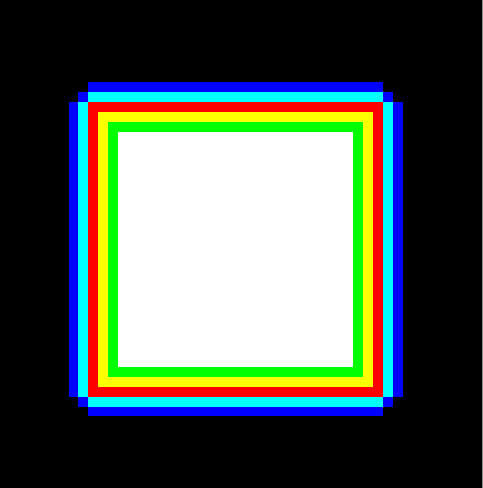
\includegraphics[width=0.8\textwidth]{../Art/WhitakerLayers.png}
 % WhitakerLayers.png: 483x488 pixel, 72dpi, 17.04x17.21 cm, bb=0 0 483 488
\end{center}
}
\only<4>{
\begin{center}
 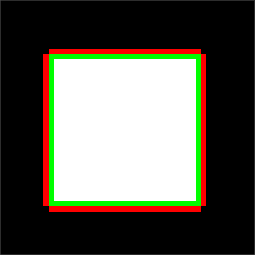
\includegraphics[width=0.8\textwidth]{../Art/ShiLayers.png}
 % WhitakerLayers.png: 483x488 pixel, 72dpi, 17.04x17.21 cm, bb=0 0 483 488
\end{center}
}
\only<5->{
\begin{center}
 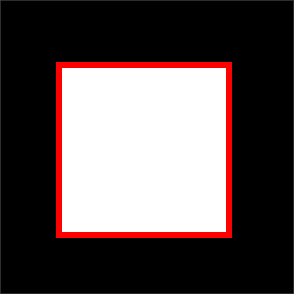
\includegraphics[width=0.8\textwidth]{../Art/MalcolmLayers.png}
 % WhitakerLayers.png: 483x488 pixel, 72dpi, 17.04x17.21 cm, bb=0 0 483 488
\end{center}
}

\end{columns}

\end{frame}

%%%%%%%%%%%%%%%%%%%%%%%%%%%%%%%%%%%%%%%%%%%%%%%%%%%%%%%%%%%%%%%%%%%%%%%%%%%%%%%%
%%%%%%%%%%%%%%%%%%%%%%%%%%%%%%%%%%%%%%%%%%%%%%%%%%%%%%%%%%%%%%%%%%%%%%%%%%%%%%%%
%%%%%%%%%%%%%%%%%%%%%%%%%%%%%%%%%%%%%%%%%%%%%%%%%%%%%%%%%%%%%%%%%%%%%%%%%%%%%%%%

\begin{frame}
\frametitle{Level Sets Equation}

\begin{columns}
  \column{0.47\textwidth} 
  \begin{block}{Term}
    \begin{itemize}
      \item Contribution for $\phi$ evolution
      \item Contribution for time step computation
      \item Coefficient
    \end{itemize} 
  \alert<2>{Easy to contribute new terms!}
  \end{block}

  \column{0.47\textwidth}
  \begin{block}{TermContainer}
    \begin{itemize}
      \item Represent a given PDEs
      \item Mix of any term
      \item Independant of the representation
    \end{itemize}
  \alert<2>{Easy to contribute new PDEs!}
  \end{block}

\end{columns}

\end{frame}

%%%%%%%%%%%%%%%%%%%%%%%%%%%%%%%%%%%%%%%%%%%%%%%%%%%%%%%%%%%%%%%%%%%%%%%%%%%%%%%%
%%%%%%%%%%%%%%%%%%%%%%%%%%%%%%%%%%%%%%%%%%%%%%%%%%%%%%%%%%%%%%%%%%%%%%%%%%%%%%%%
%%%%%%%%%%%%%%%%%%%%%%%%%%%%%%%%%%%%%%%%%%%%%%%%%%%%%%%%%%%%%%%%%%%%%%%%%%%%%%%%

\begin{frame}
\frametitle{Other Features}
  \begin{itemize}
    \item N Level-Sets function evolving at the same time
    \item Geometrical Constraints
  \end{itemize}
\end{frame}


